\chapter{相关工作}
本文研究基于弱标签和噪声标签的弱监督语义分割,在基于弱标签的语义分割中,我们的研究重点是如何结合形状先验,在基于噪声标签的语义分割中,我们关注如何利用图像结构和标签联系。本章分别介绍基于弱标签和噪声标签的语义分割的相关工作。在基于弱标签的分割学习中,为了在缺少完整训练数据的条件下学习形状先验,我们还介绍了自学习方法和去噪自编码器的工作。

\section{基于弱标签的语义分割}

我们先在~\ref{sec:rel_wss}节介绍通常的基于弱标签的语义分割的相关工作,它们通过标签传播或先验约束取得了一些进展,但鲜有工作探索结合形状先验的方向。本文目标是设计方法从弱标签中学习物体的形状先验,用于分割形状去噪。为了解决形状学习中训练数据缺乏的问题,我们在~\ref{sec:rel_stl}节总结了自学习方法;为了根据形状先验来学习去噪能力,我们在~\ref{sec:rel_dae}节总结了降噪自编码器的相关工作。

\subsection{基于弱标签的分割学习} \label{sec:rel_wss}

为了降低标注成本,基于弱标签的语义分割采用粗粒度的标签,比如图像级标签(\cite{wang2020self,fan2020learning,chang2020weakly}),边界框(\cite{papandreou2015weakly,khoreva2017simple,song2019box})和涂鸦式标签(\cite{lin2016scribblesup,vernaza2017learning,tang2018regularized})。这些弱标签的标注成本远低于完整标签,研究该任务对提高数据标注的利用效率有重要意义。现有的方法大致可以分为两类,第一类采用迭代学习的框架,即先传播监督信息,生成伪标签,再用其训练模型。第二类方法应用基于正则项的端到端训练框架,避免了生成伪标签的过程。接下来我们对这些工作进行详细介绍。


\citet{papandreou2015weakly}探索了在边界框和图像级标签这样的训练数据的学习算法。该工作为弱监督的语义图像分割模型训练开发了期望最大化方法,来解决模型训练不足的问题。在标签标注成本上,收集图像中每个类别周围的边界框标注会比逐像素标注快大约15倍\citep{lin2014microsoft},而收集图像级标签的标注成本更少。该文作者提出的期望最大化方法,在估计(被弱标签约束的)像素标签和用随机梯度下降方法优化深度网络参数这两个阶段交替进行。

在图像级标签上,作者定义了该问题的概率图模型,并根据该模型,用期望最大化算法来从训练数据中学习模型参数,如图~\ref{c2_fig1}。考虑求期望阶段偏置(bias)的不同形式,作者提出了两种具体方法:EM-Fixed 和 EM-Adapt。在 EM-Fixed 中,根据图像级标签为每个像素设置固定的概率偏置,施加图像的前景区域约束。在 EM-Adapt 中,根据图像级标签设定前景区域面积的偏置,来对前景区域施加约束。

在边界框标签上,作者也探索了三种方法来训练分割模型:Bbox-Rect, Bbox-Seg 和 Bbox-EM-Fixed,如图~\ref{c2_fig2}。Bbox-Rect 采用了简单的标签赋值方法,在边界框内的像素全部设为目标类别的标签,在其外的则为背景标签。这种简单的方法会引入一些边界框内的假正类标签,为了解决这一问题,Bbox-Seg 被提出。具体做法是,在边界框内不再全部设为正类标签,而是选择一定比例的边界框中心区域设为正类标签,边界框外则全部设为负类标签,然后构建一个条件随机场来推理其他的标签。这两种利用边界框来估计分割图标签的方法,都可以看作前处理步骤,随后利用生成标签来训练分割网络。此外,作者还提出了 Bbox-EM-Fixed,目标是在训练中改进分割标签估计,这是 EM-Fixed 的一个变种,不同的是仅对边界框内的像素施加前景偏置。最后这篇文章在 PASCAL VOC 2012 图像分割基准的评价指标有较高提升,验证了这些方法的有效性。


    \begin{figure*}[tbp]
        \centering 
        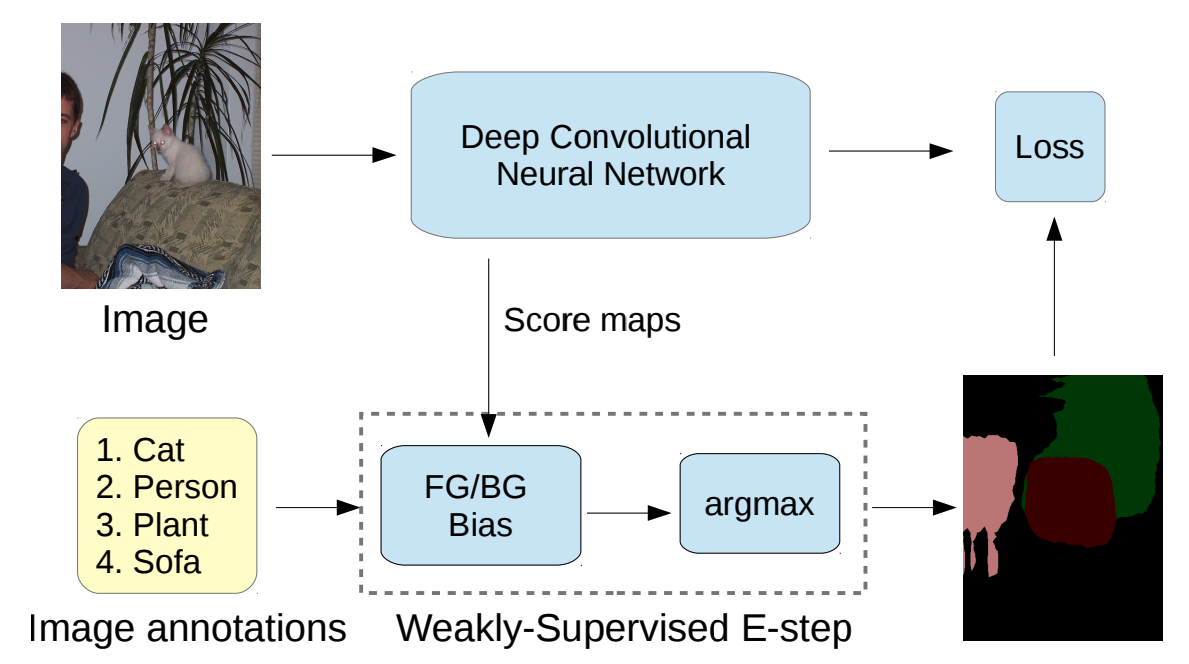
\includegraphics[width=1.0\textwidth]{img/c2/rel_a1.png}
        \bicaption{使用图像级标签的 DeepLab 模型训练过程。图自~\citet{papandreou2015weakly}。}{DeepLab model training using image-level labels. Figure is from~\citet{papandreou2015weakly}.}
        \label{c2_fig1}
    \end{figure*}

    \begin{figure*}[tbp]
        \centering 
        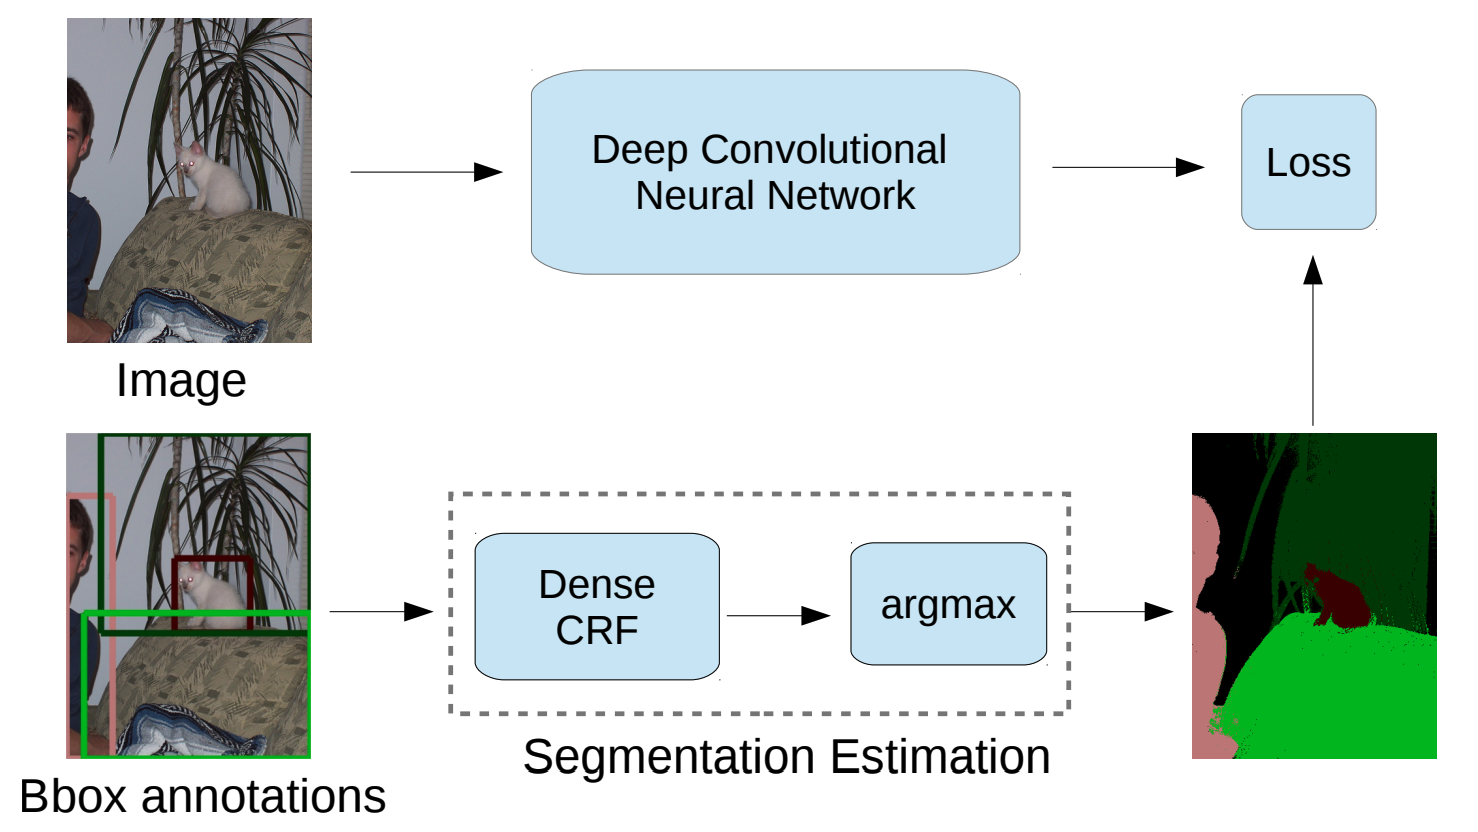
\includegraphics[width=1.0\textwidth]{img/c2/rel_a2.png}
        \bicaption{使用边界框标签的 DeepLab 模型训练过程。图自~\citet{papandreou2015weakly}。}{DeepLab model training from bounding boxes. Figure is from~\citet{papandreou2015weakly}.}
        \label{c2_fig2}
    \end{figure*}

    \begin{figure*}[tbp]
        \centering 
        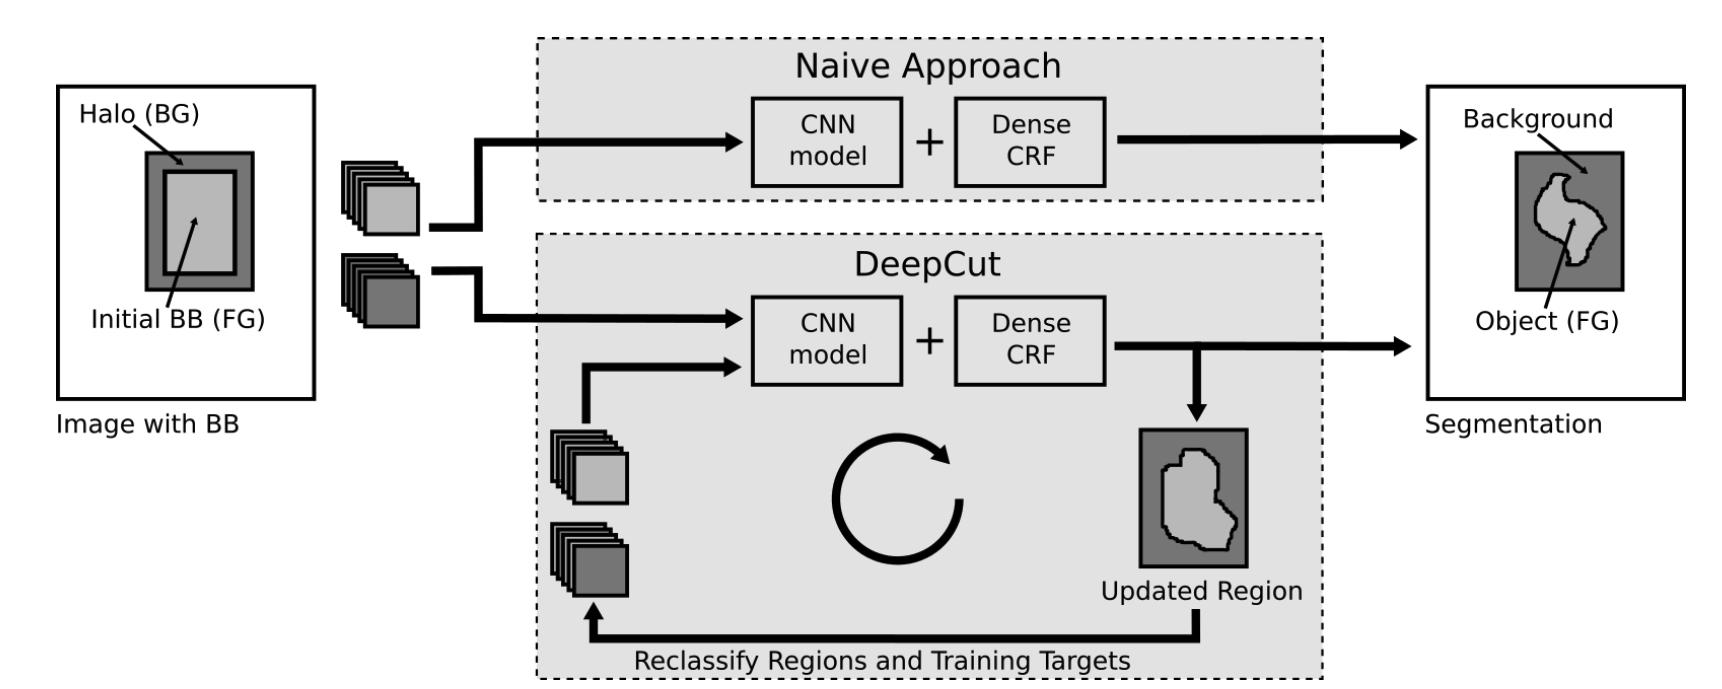
\includegraphics[width=1.0\textwidth]{img/c2/rel_a3.png}
        \bicaption{普通的 CNN 学习与提出的 DeepCut 方法的对比,后者迭代地更新学习目标。图自~\citet{rajchl2016deepcut}。}{Naive CNN learning versus the proposed DeepCut approach, iteratively updating the learning target classes for input patches. Figure is from~\citet{rajchl2016deepcut}.}
        \label{c2_fig3}
    \end{figure*}

    \begin{figure*}[tbp]
        \centering 
        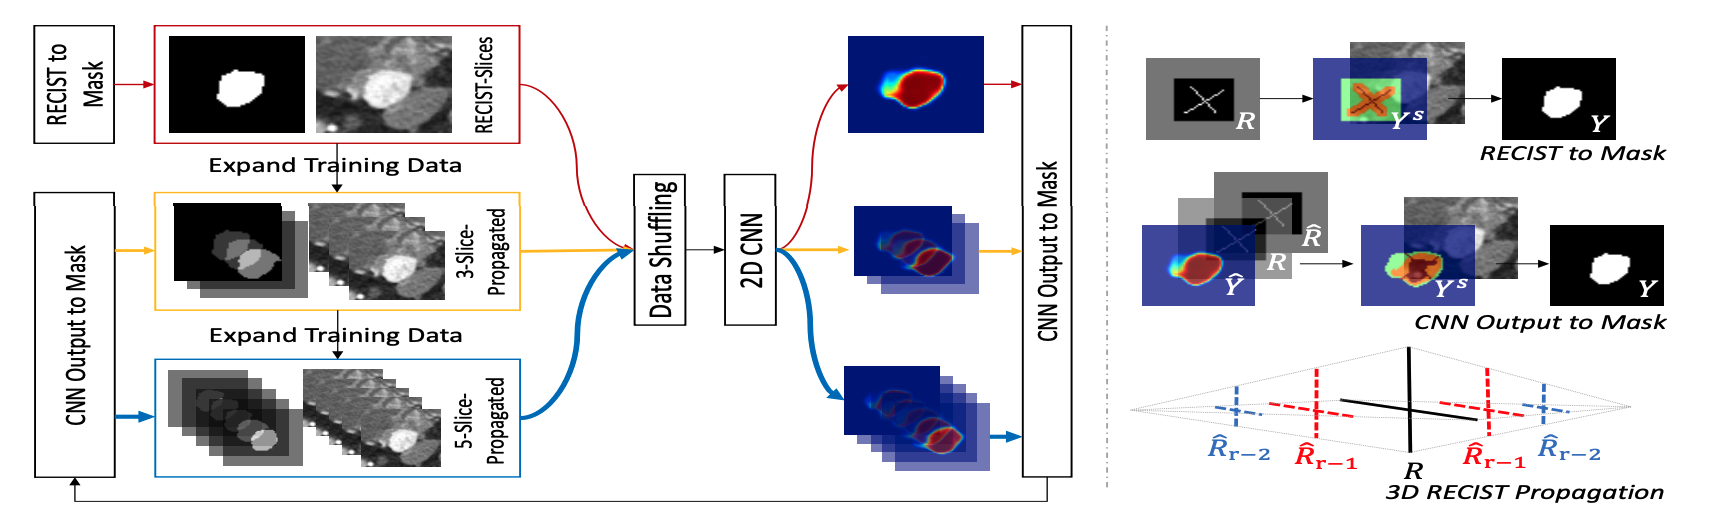
\includegraphics[width=1.0\textwidth]{img/c2/rel_a4.png}
        \bicaption{逐切片扩张的三维图像分割网络。图自~\citet{cai2018accurate}。}{The overview of slice-propagated 3D image segmentation network. Figure is from~\citet{cai2018accurate}.}
        % 左侧图展示了训练图像的增加过程,每次邻近的图片连通生成的弱标签一起加入训练。右侧图展示了弱标签的传播过程,RECIST 标签通过 GrabCut 传播,未标注图像通过分割网络的预测传播得到标签。
        % Left: Each time adjacent slices are fed into the training process. Right: RECIST labels are initialized by GrabCut method, and CNN outputs are used to gradually generate extra training data for lesion segmentation.
        \label{c2_fig4}
    \end{figure*}


    \begin{figure*}[tbp]
        \centering 
        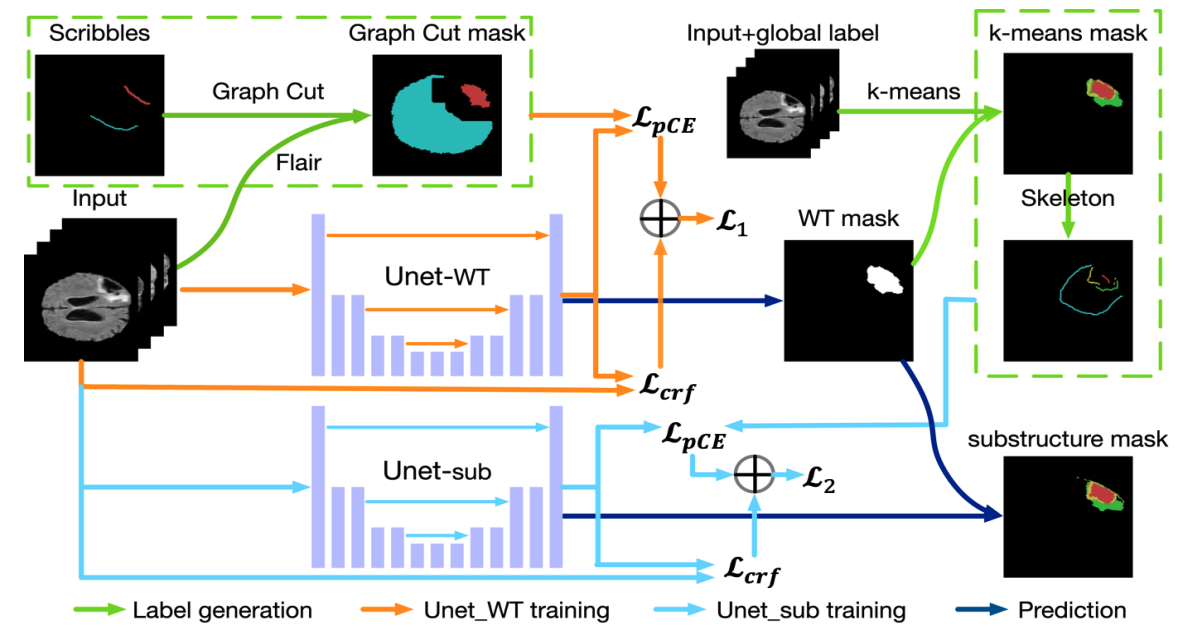
\includegraphics[width=1.0\textwidth]{img/c2/rel_a5.png}
        \bicaption{级联训练分割网络。图自~\citet{ji2019scribble}。}{Workflow of the proposed cascaded method. Figure is from~\citet{ji2019scribble}.}
        \label{c2_fig5}
    \end{figure*}


在 Deepcut\citep{rajchl2016deepcut}中进一步探讨了迭代地更新训练目标标签和模型参数的思想。该文的研究重点在边界框标签上。作者首先指出了边界框标签相对其他形式(比如涂鸦式)的优势,即对问题的空间约束(目标物体是完全包含在边界框内的),快速标注和轻量级存储(只需要定义对角线的两个端点)。本文目标是把神经网络模型和迭代的图优化方法相结合,以从粗粒度的边界框标签恢复像素级物体分割。受 GrabCut 方法的启发,其用一个基于像素强度的图模型迭代地拟合图像区域,随后被正则化以得到分割。该文将此任务定义为稠密连接的条件随机场下的能量最小化问题,提出迭代地更新训练目标,并且应用全连接条件随机场来规范分割。
模型结构如图~\ref{c2_fig3},作者对比了普通的 CNN 训练方法和提出的 Deepcut 迭代方法。重要的区别在于,Deepcut 对训练目标的迭代更新,可以渐进地提高模型训练的效果,这种迭代提高的方法要优于单一不变的训练目标。具体实现上,论文中还提出了DeepCut方法的变体,并与其它算法在弱监督任务进行了比较。Deepcut 方法在 Fetal Magnetric Resonance Dataset\citep{damodaram2012foetal}的这两个分割任务上取得了不错的精度,超过了之前的方法。

很多医学图像数据都是三维形态的,相比于二维图像,其标注成本大幅提高,因此基于弱标签的分割方法更为重要。三维图像可以直接处理,也可以分解为一系列连续的二维医学图像进行处理。
在三维图像上,\citet{cai2018accurate}研究利用现有的 RECIST直径 标签来生成完整的三维图像分割结果。三维图像的 RECIST 标签只在中心一张二维切片上(RECIST 标签是在中心切片的物体内部画出一对相互垂直的长轴与短轴),这篇文章要解决两个主要挑战,一是有弱标注图像的标签传播,以训练有效的分割网络,二是从已标注图像到未标注图像的标签传播,来分割出完整的三维物体。对前一个问题,作者采用无监督方法来初始化标签,对后一个问题,则利用分割网络的预测结果,来自动生成可信的标签。作者用一个迭代扩张训练图像的过程,来覆盖整个待分割的三维图像。总的来说,这篇文章把三维图像分割分解成一系列二维图像分割任务,通过标签传播和分割模型的分阶段训练来生成分割结果,最后堆叠组合为三维分割。分割过程如图~\ref{c2_fig4}所示,是一个基于卷积神经网络的逐切片传播的分割方法。首先,为有 RECIST 标注的切片初始化分割标签,然后用这些切片训练分割模型。其后,利用初步训练的模型给临近的未标注切片初始化分割标签,用扩张后的切片及标签继续训练模型。这个过程不断迭代,直至所有切片都加入训练。作者在淋巴结数据集\citep{roth2014new}和 DeepLesion 数据集\citep{yan2018deep}进行实验,表明了所提出方法的优良性能。

另外,有些组织由多个子区域构成,比如脑肿瘤可能包括两到三种子区域,每个子区域都需要单独分割。如果每个子区域进行完整标注,耗时而低效。\citet{ji2019scribble}为这种任务提出了一种结合两种弱标签形式的标注方法,来减少标注成本。这种混合标注策略是,对整体的肿瘤区域用涂鸦式标签,而对各个子区域给出全局图像级标签。这种方式下,整体的肿瘤区域通过涂鸦式标签来学习,图像级标签用来引导子区域的聚类。这篇文章提出通过级联模型的方式,来解决这样具有层次结构的分割任务。
模型如图~\ref{c2_fig5}。受之前的级联网络的启发,这个模型采用先训练整体肿瘤分割,再子区域分割的方式。具体地,作者先用涂鸦式标签和由其初始化得到的图割标签,来训练整体肿瘤的分割网络。之后再在图像级标签的引导下,用无监督聚类方法提取肿瘤的各个子区域。最后把聚类得到的标签作为弱标签,来训练第二个子区域分割网络。作者还在分割网络训练中加入了 Dense CRF Loss,来提高分割边缘的连续性与准确性。这种方法在 BraTS2017 数据集\citep{menze2014multimodal}上进行了评估,在整体肿瘤分割和子区域分割上都取得了接近全监督上限的结果。

以上方法有共同之处:都是利用推理方法(GrabCut、CRF或初始化模型推理)来显式地生成伪标签,然后经处理后作为训练目标来优化模型。除了显式生成伪标签再训练,另一类方法直接使用弱标签训练,通过施加先验正则项来约束训练,以求较好的训练结果。\citet{kervadec2020bounding}和 \citet{tang2018regularized}是近期的重要工作。

\citet{kervadec2020bounding} 采用边界框标签,提出了一种基于全局约束的弱监督分割方法。作者首先提出了边界框的拓扑先验,包括框内的紧致性先验、框外的全背景先验和前景区域尺寸先验,这些先验被作为约束条件加入模型的训练目标。不过这些先验是不等式形式的约束,为了直接训练,作者通过对数障碍惩罚函数把不等式约束处理为损失函数的形式。这种利用全局约束来解决弱监督问题的方法,充分利用了领域先验知识,避免了只有少量标签训练的结果不确定性。并且基于约束方法能实现端到端的训练,可以避免显式生成伪标签过程中的错误传播。
    \begin{figure*}[tbp]
        \centering 
        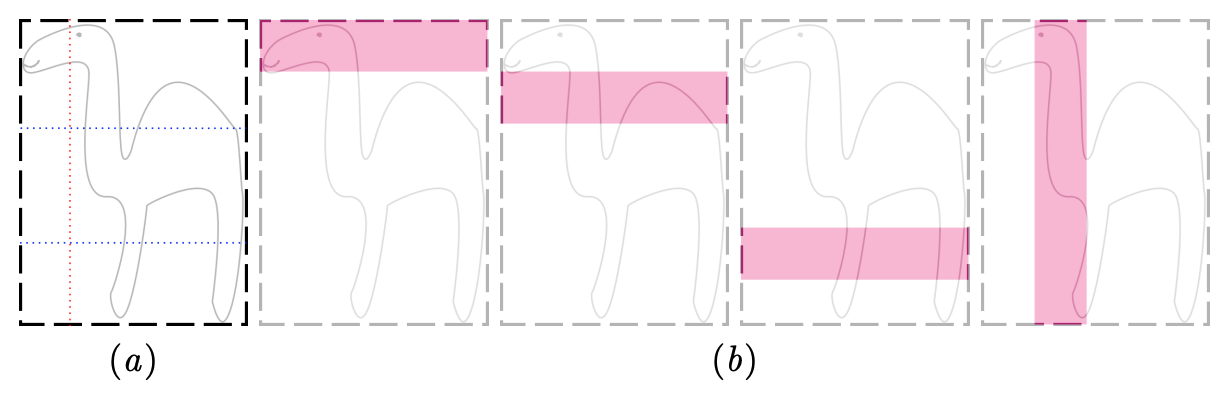
\includegraphics[width=1.0\textwidth]{img/c2/rel_a6.png}
        \bicaption{边界框标签的紧致性先验示意图:(a) 任一条竖直或水平的线段至少与一个前景像素相交。 (b) 更广泛地,宽度为 w 的线段至少与 w 个前景像素相交。图自~\citet{kervadec2020bounding}。}{Illustration of the tightness prior: (a) any vertical (red) or horizontal (blue) line will cross at least one pixel of the camel. (b) This can be generalized, where segments of width w cross at least w pixels of camel. Figure is from~\citet{kervadec2020bounding}.}
        \label{c2_fig6}
    \end{figure*}
全局约束充分考虑利用弱标签的信息。紧致性先验如图~\ref{c2_fig6}所示,基于边界框紧致地包围着目标物体边界,在框内的任意一条水平或竖直线段都会至少与一个前景像素相交。这种先验约束,能够防止训练过程中过拟合到背景类别而前景预测失败的问题。全背景先验是指边界框外的区域都属于背景类别,约束了前景的空间区域。前景区域尺寸先验,则是指目标物体在框内的面积比例有先验的下界与上界,利用尺寸先验可以约束分割结果的区域比例关系。这些全局先验通过对数障碍惩罚函数转换为标准的损失函数形式,可以直接使用随机梯度下降方法进行优化。
这篇文章在两个不同的公开数据集 PROMISE12\citep{Litjens2014EvaluationOP}和 ATLAS\citep{Liew2018ALO}进行试验,结果表明,这种方法可以接近全监督的分割效果,并且显著超过之前的 DeepCut 方法,同时避免了显式生成伪标签的耗时计算。

\citet{tang2018regularized}则在涂鸦式标签上探索把正则项融入损失函数,以实现在训练中结合浅层分割的效果(如图割法或 Dense CRF)。这篇文章通过设计 MRF/CRF 形式的约束项,来为分割模型引入浅层分割的特性如连续性、相关性、空间关系等。这种隐式的约束方法简化了弱监督的训练,避免了额外的 MRF/CRF 推理步骤来生成伪标签,提高了训练的质量和效率。这篇文章提出了几种用于弱监督的正则损失,分别是基于 Potts、Dense CRF 和 Kernelcut 的正则。作者通过 PASCAL VOC12\citep{everingham2015pascal} 的实验对比了之前的生成伪标签的方法和不同正则损失函数,验证了所提出方法在弱监督语义分割的接近全监督的效果。


\subsection{自学习方法} \label{sec:rel_stl}
学习任务中,训练数据的缺乏是很常见的困难,而自学习方法(self-taught learning)可以作为一种解决方案。
自学习方法一般使用未标注的数据集进行训练,不同于自监督学习(self-supervised learning)中使用自身信号作为训练目标,自学习方法使用与目标任务一致的训练目标。\footnote{另一个区分的概念是自训练(self-training)方法,这是半监督学习中的一种方法,它要求有一定数量的数据标注,而自学习方法没有这样的假设。}
因此,训练数据及标签产生、学习方法是其中考虑的重要方面。近期的工作将自学习方法应用于分类任务\citep{raina2007self,wang2013robust,feng2020autoencoder}、聚类任务\citep{li2017self,dai2008self}和定位任务\citep{bazzani2016self,jie2017deep},较好地利用了未标注数据进行训练,并随之提高目标任务的性能。我们考虑将自学习方法引入到弱监督语义分割中,解决形状先验的学习问题。就我们所知,迄今还没有工作探索过类似的方向。本节详细介绍一些运用自学习方法的相关工作。

在分类任务上,\citet{raina2007self} 通过在未标注数据集上应用自学习方法,利用学到的特征表示来提升在给定数据集的分类性能。自学习方法所使用的未标注数据集不受目标任务的限制。这篇文章出于对图像相似的基本视觉模式(如边缘模式)的观察,尝试从未标注数据中学习到简洁的、高阶特征的表示,这种表示可以使目标分类任务更容易。
具体地,作者所提出的自学习方法包括两个阶段。首先,在未标注数据上定义用稀疏编码构建高阶特征的优化问题,通过解这样的优化问题,可以得到图像的稀疏高阶表示。图~\ref{c2_fig7}展示了从图像块学习到的稀疏编码基向量,每个方格表示一种基。然后,这种已被学到的表征可以被应用于不同的分类任务,提高目标任务的效果。
    \begin{figure*}[tbp]
        \centering 
        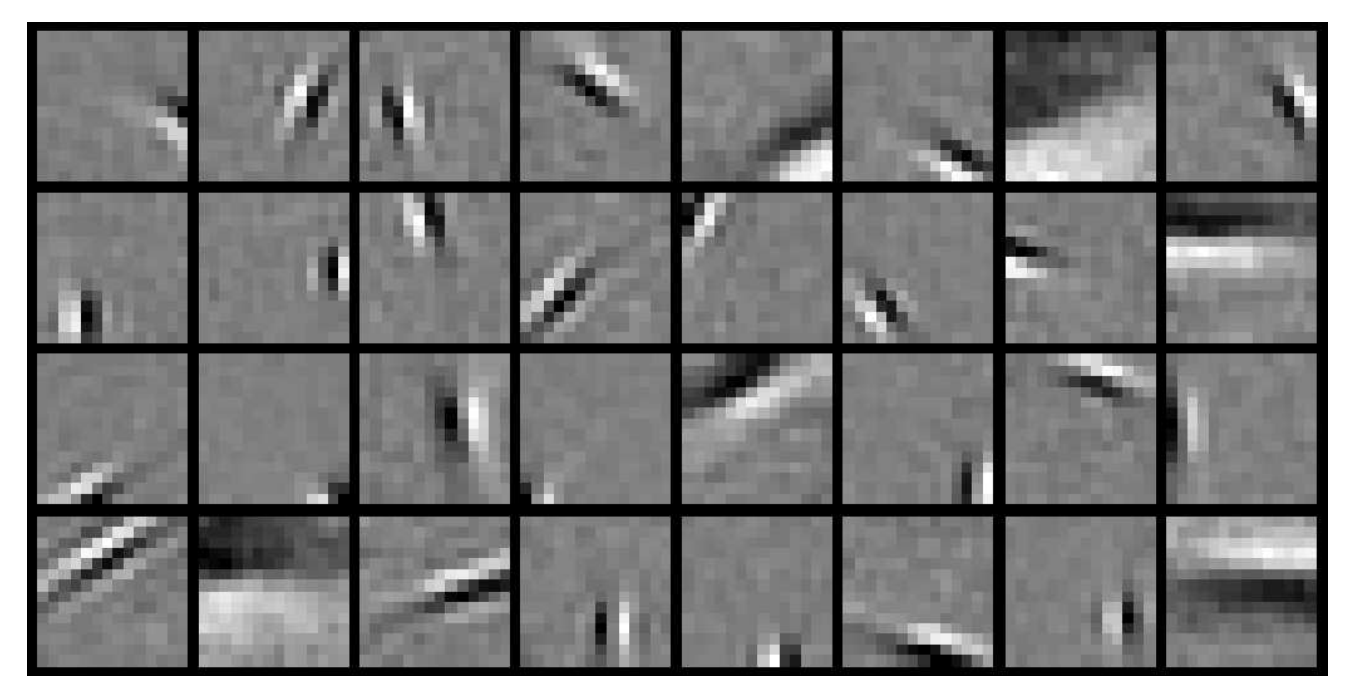
\includegraphics[width=1.0\textwidth]{img/c2/rel_b1.png}
        \bicaption{从图像块学习到的稀疏编码基向量的例子。图自~\citet{raina2007self}。}{Example sparse coding bases learned from image patches. Figure is from~\citet{raina2007self}.}
        \label{c2_fig7}
    \end{figure*}

在聚类任务上,\citet{li2017self} 观察到之前的自学习方法通常会忽略数据中的结构信息,因此专注于建立一个自学习编码框架,它可以有效地利用从辅助数据集抽象出来的丰富的低级模式信息,来描述目标数据集的高级结构信息。通过利用从辅助域和目标域中学习到的高质量字典,该方法为目标域中的样本学习了特征丰富的编码。由于许多类型的视觉数据已被证明包含子空间结构,作者在编码目标中引入了低秩约束,以更好地描述给定目标集的结构。这种提出的自学习的低秩编码框架,被形式化为一个非凸的秩最小化和字典学习问题。
模型框架如图~\ref{c2_fig8}。目标域的一个小数据集不足以提取有效的特征,通过利用辅助域的数据集,模型学习到一个共享字典,并对目标域的系数矩阵施加低秩约束,产生新的特征表示。随后这种特征表示作为图像聚类或分类任务的输入,提升训练性能。
    \begin{figure*}[tbp]
        \centering 
        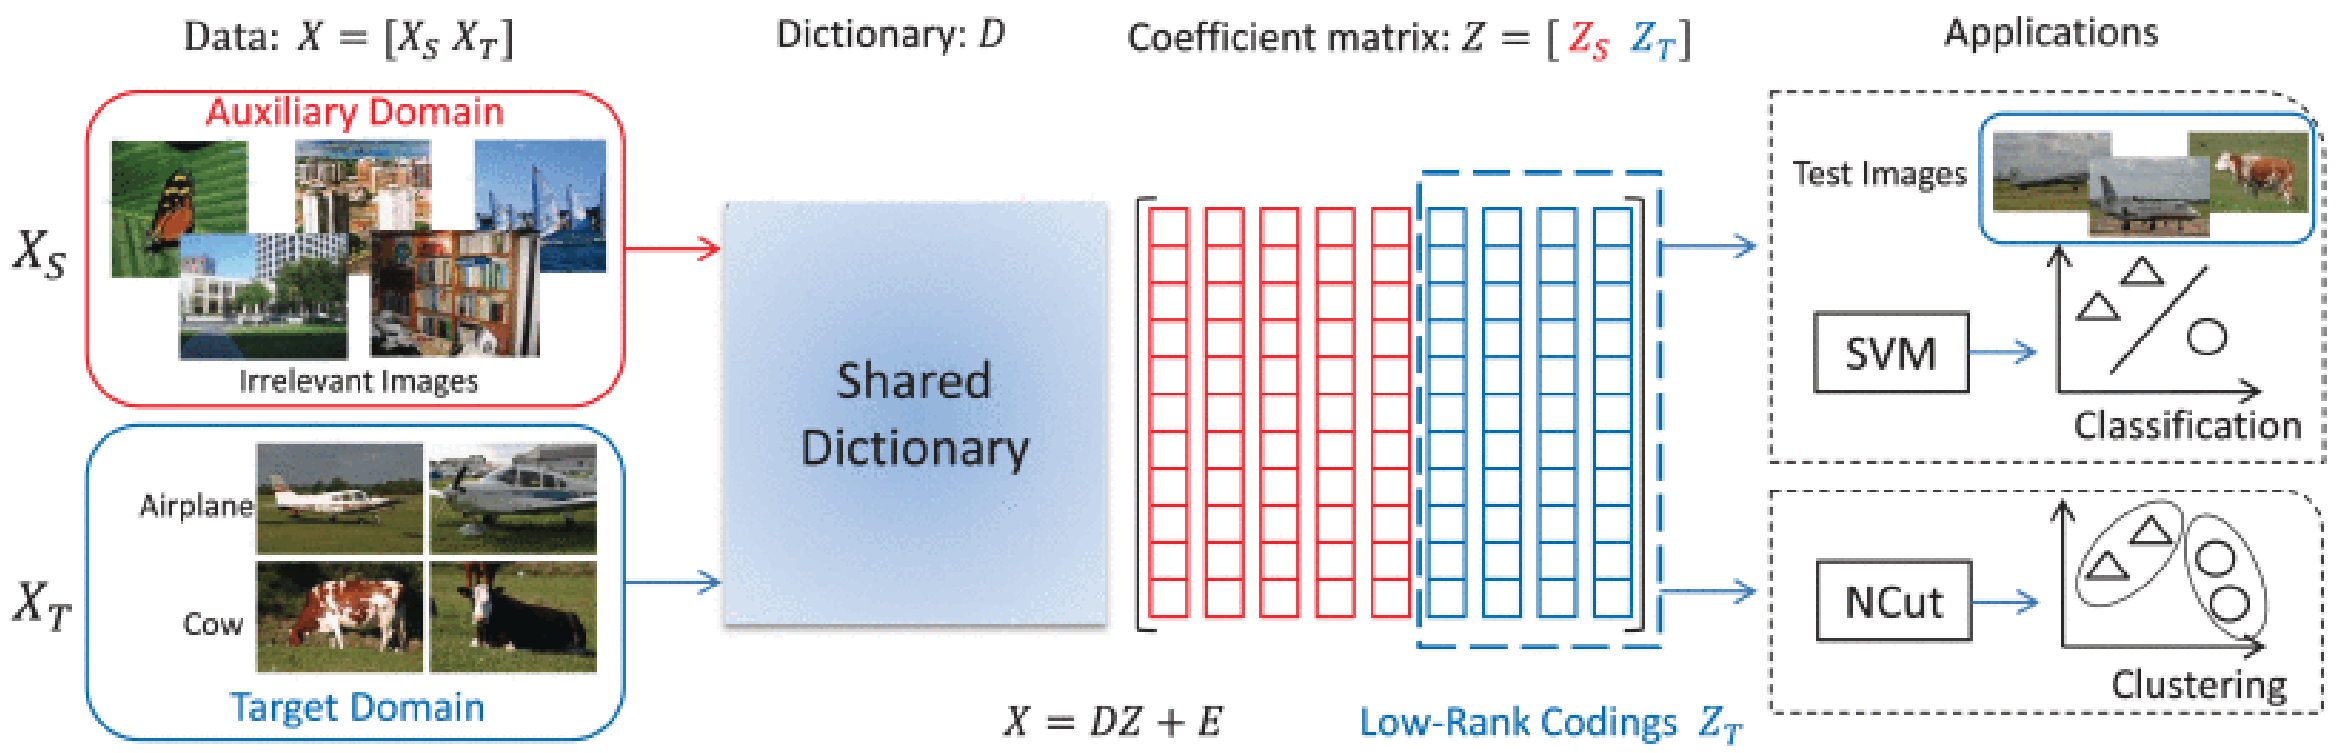
\includegraphics[width=1.0\textwidth]{img/c2/rel_b2.png}
        \bicaption{自学习的低秩编码模型。图自~\citet{li2017self}。}{Diagram of the S-Low coding framework. Figure is from~\citet{li2017self}.}
        \label{c2_fig8}
    \end{figure*}

在定位任务上,\citet{bazzani2016self} 设计了自学习的物体定位方法,不需要求真实的的边界框标签。其关键思想是,当人为遮挡图像的不同区域时输出的类别识别概率会变化,分析这种变化可以找到包含该物体的区域。图~\ref{c2_fig9} 描述了部分遮蔽出的图像在卷积网络的传播,从而影响识别概率的过程。
这种思想被融入到分层聚类方法,产生自学习的边界框标签。
    \begin{figure*}[tbp]
        \centering 
        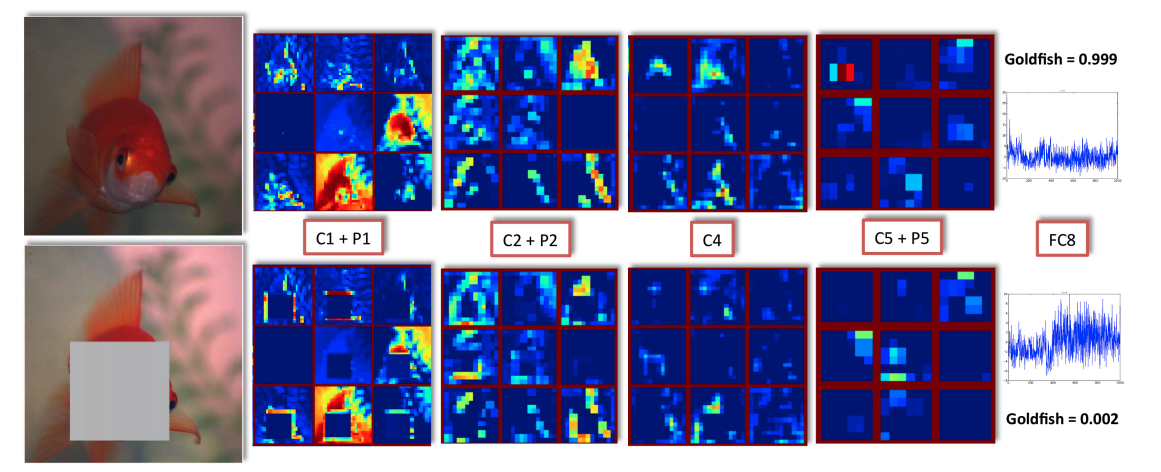
\includegraphics[width=1.0\textwidth]{img/c2/rel_b3.png}
        \bicaption{原图像(第一行)、被遮挡的图像(第二行)以及它们在卷积网络的各层输出。图自~\citet{bazzani2016self}。}{The image (first row), its mask-out version (second row) and the outputs of different layers of the convolutional network. Figure is from~\citet{bazzani2016self}.}
        \label{c2_fig9}
    \end{figure*}
这篇文章提出的物体定位方法在准确率和召回率上都优于之前的方法,在 ILSVRC-2012 数据集\citep{russakovsky2015imagenet}上比之前最好的方法有大幅的提升。并且,自学习方法生成的标签用于训练定位模型,定位结果与真实标注的训练结果非常接近。

\subsection{去噪自编码器} \label{sec:rel_dae}
去噪自编码器目标是将输入图像编码到高维空间的一个隐向量,该向量对噪声具有不变性,作为原始图像的鲁棒表示。近来有一些工作应用去噪自编码器来产生更好的图像表征和对输入的抗干扰能力。
\citet{vincent2010stacked} 探索构建一种基于堆叠的去噪自编码器的深度网络,来提高模型的泛化性与分类准确率。这些自编码器经过训练,具有对被噪声干扰的输入图像进行去噪的能力。这种网络表现出明显的低分类误差,这种以无监督方式学习的高层次语义表征也有助于提高后续 SVM 的性能。
具体地,图~\ref{c2_fig10}是去噪自编码器的结构。原始输入样本被随机地做噪声增强,然后通过自动编码器映射到隐向量,再通过自动解码器重建输入样本,重建损失函数由重建样本与原始样本的误差衡量。这种训练方式使模型具有了去噪和恢复原始干净样本的能力。这项工作表明了无监督任务目标中,去噪目标对学习一个有用的高阶表征的指导意义。
    \begin{figure*}[tbp]
        \centering 
        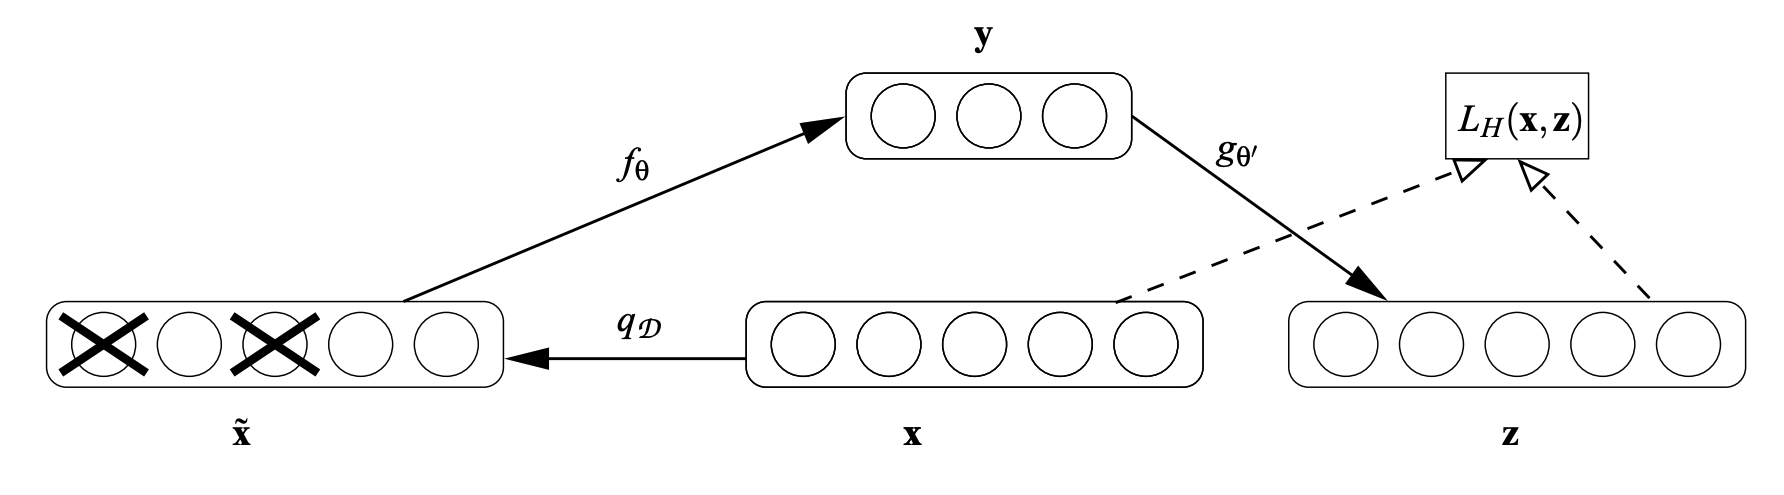
\includegraphics[width=1.0\textwidth]{img/c2/rel_b4.png}
        \bicaption{去噪自编码器的结构。图自~\citet{vincent2010stacked}。}{The denoising autoencoder architecture. Figure is from~\citet{vincent2010stacked}.}
        \label{c2_fig10}
    \end{figure*}

在三维姿态估计中,为了解决之前工作中对物体遮挡等动态变化、训练数据不足等挑战,\citet{Sundermeyer_2018_ECCV} 提出一种全新的基于增强型去噪自编码器的三维方向估计模型,并在使用域随机化的三维模型的增强视图上训练。增强型自编码器如图~\ref{c2_fig11},原始输入图像首先通过数据增强,产生几何结构和颜色增强后的图像,作为自动编码器的输入,输出的目标是回复原始输入图像。这种增强型自动编码器可以使模型具备动态环境下恢复准确姿态的能力,优点是:不需要真实的有姿态标签的数据,可以通用于多重测试传感器;不需要学习从输入图像到物体姿态的显式映射,而是采用样本隐空间的姿态隐式表示。基于此的姿态估计在 T-LESS 数据集~\citep{hodan2017t}和 LineMOD 数据集~\citep{hinterstoisser2011multimodal}都取得了先进的性能。
    \begin{figure*}[tbp]
        \centering 
        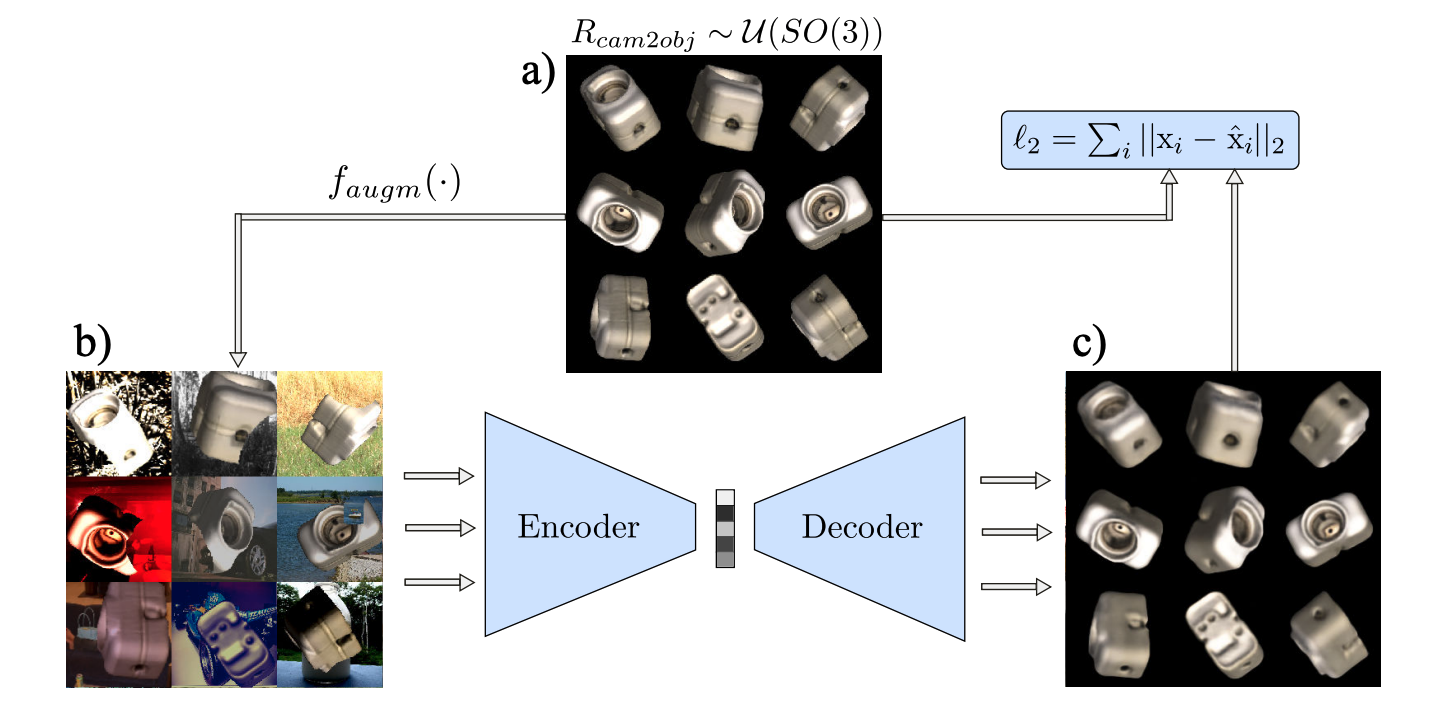
\includegraphics[width=1.0\textwidth]{img/c2/rel_b5.png}
        \bicaption{增强型去噪自编码器的结构和训练过程。图自~\citet{Sundermeyer_2018_ECCV}。}{Augmented Autoencoder and its training process. Figure is from~\citet{Sundermeyer_2018_ECCV}.}
        \label{c2_fig10}
    \end{figure*}

\section{基于噪声标签的语义分割}
基于噪声标签的语义分割作为弱监督的另一种类型,面临着训练标签中有一部分错误的问题。如何有效利用好噪声标签,来训练得到鲁棒的语义分割网络,是该任务的核心问题。近来已有一些工作\citep{Zhu2019PickandLearnAQ,Xue2020CascadedRL,Zhang2020CharacterizingLE,Zhang2020RobustMI},在该任务上做了探索,并取得了一些进展。

对噪声标签的利用,需要模型具备评估标签质量的能力,以决定使用或丢弃哪些标签。正确的标签可以让模型充分训练,而噪声标签会干扰训练结果,甚至由于深度神经网络的较强的表征能力,模型会记住这些标签错误。除了设计方法尽可能选出正确标签来学习,另一方面,根据训练过程中学到的信息,错误标签也可以被纠正为正确标签,带来进一步的性能提升。

\citet{Zhu2019PickandLearnAQ} 在分割网络中引入了标签质量评估策略,来自动评估每张图像的标签质量,随后利用正确的标签进行训练。这篇文章提出了一个分割网络,其自动评估训练集里标签的相对质量,并使用好的标签来更新网络参数。自动评估的想法来自于标签与输入图像的一致性关系,噪声标签往往与输入样本有明显的冲突,这区别于同一批次中对比正确标签与输入样本的关系。此外还设计了一个过拟合控制模块,让网络在训练过程中尽可能地从精确标签中学习。过拟合控制模块可以确保有足够的可训练样本和避免过拟合。
    \begin{figure*}[tbp]
        \centering 
        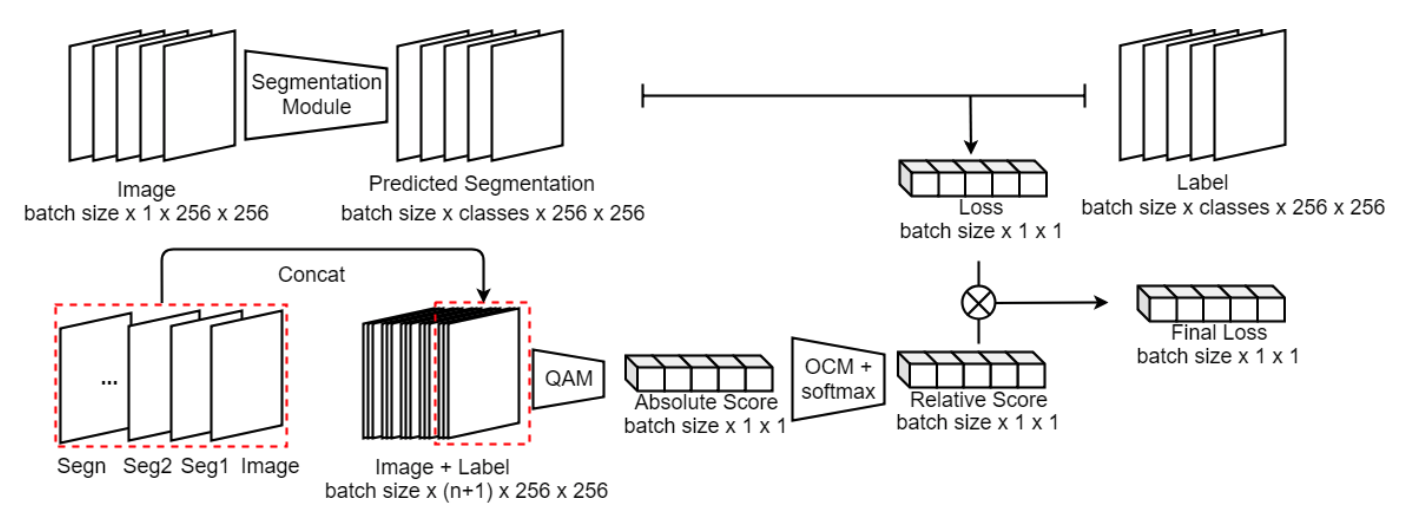
\includegraphics[width=1.0\textwidth]{img/c2/rel_c1.png}
        \bicaption{应用标签质量评估策略的端到端分割模型。图自~\citet{Zhu2019PickandLearnAQ}。}{The end-to-end architecture of the proposed label quality evaluation strategy. Figure is from~\citet{Zhu2019PickandLearnAQ}.}
        \label{c2_fig11}
    \end{figure*}
模型结构如图~\ref{c2_fig11}所示,该工作的中心目标是使用网络来计算同一批次中图像的相对质量分数,并找到存在于噪声标签中的冲突信息,利用这些信息,网络可以将噪声标签和正确标签区分开来。该模型由三个组成模块:分割模块、质量评估模块和过拟合控制模块。
训练过程中,与有正确标签的样本相比,有噪声标签的样本的预测分割会有较高的损失值,直接训练会干扰模型的学习能力和效果。为了对同一批次样本进行重新加权,质量评估模块和过拟合控制模块联合为每个输入产生相对权重,这个权重与分割模块计算的损失相乘,作为最终损失进行反向传播。这样,正确标签和噪声标签对模型的训练有不同权重的影响,使得模型能进行正确训练且具备抗噪声干扰能力。
分割模块是通用的生成语义分割的卷积神经网络,用以将输入图像通过多层特征提取和分辨率恢复产生分割预测。
质量评估模块也是一个卷积网络,但它将输入图像及其标签的拼接作为输入,为每张图像输出一个对应的质量评估分数,与分割模块平行运行。
过拟合控制模块在质量评估模块之后,为了防止前一个模块输出的评估分数的过拟合问题,以保证模型的训练稳定。它通过一个重缩放变换来调整评估分数。
在公开的生物医学分割 JSRT 数据集~\cite{Shiraishi2000DevelopmentOA}的实验表明,该方法优于基线方法,并且在不同的噪声水平下都能保持较高的准确性和良好的泛化能力。


为了更充分地利用标签信息,\citet{Xue2020CascadedRL} 提出了一种新的级联式的鲁棒学习框架。模型由三个独立的网络结构组成,这种设计能够从同级网络中有效学习信息。该框架包含两阶段,第一阶段通过模型选择机制选出正确标签的图像样本,通过分割损失最小化来训练网络。第二阶段则设计了一个带标签校正的联合优化框架,以逐步纠正错误标签并改进网络性能。
    \begin{figure*}[tbp]
        \centering 
        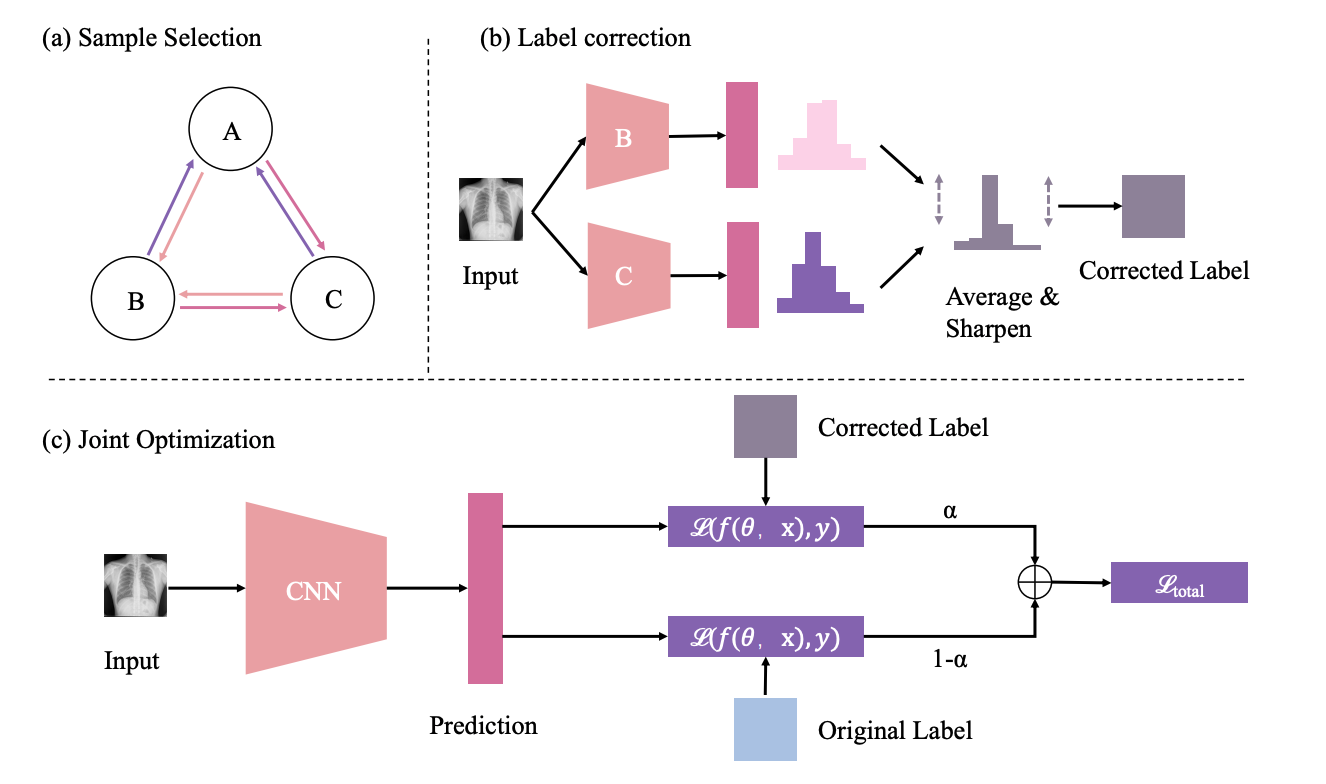
\includegraphics[width=1.0\textwidth]{img/c2/rel_c2.png}
        \bicaption{级联式鲁棒学习框架。图自~\citet{Xue2020CascadedRL}。}{Illustration of the pipeline of our cascaded robust learning framework. Figure is from~\citet{Xue2020CascadedRL}.}
        \label{c2_fig12}
    \end{figure*}
如图~\ref{c2_fig12},作者沿用了之前的鲁棒学习思路:选用高置信度的样本来更新网络可以提高对噪声标签的鲁棒性。所提的框架由三个独立而相同结构的网络组成。在第一阶段的训练过程中,选择不确定性较小的高置信样本来更新每个网络,因为这些样本大概率是正确标签。具体地,每个网络用于训练的样本由其他两个网络获得,首先排除预测结果不一致的样本,然后在低不确定性样本中,选择小损失值的样本。
然而,样本选择阶段只有部分样本可以用于训练,而无法充分利用标签信息。为了提高标签的利用效率,第二阶段设计了一个联合优化框架,用原始标签和修正标签共同训练网络。为了纠正有噪声的标签,作者设计了一个标签校正模块,校正标签由不同网络预测的平均值再通过锐化函数生成。
总之,通过这样一种级联的学习框架,这篇工作充分利用了噪声标签的信息,且避免了错误标签的干扰,提高了分割的准确性。
% 这篇工作在深圳医院收集的公开胸部 X 射线数据集进行了实验,结果表明,相比于之前的方法,这种基连的鲁棒学习框架在分割任务的准确性

% \citet{CL}

上述两篇工作都可以视为图像级别的的训练加权策略,这类方法将每幅图像的标签视为正确或噪声,并迭代选择或重新权衡图像样本。但是在重度的噪声环境下鲁棒性很差,因为它们无法充分利用每幅图像中具有正确注释的像素,为了解决这一局限性,另一类方法是将分割任务视为像素级的分类任务,进行像素级样本选择或标签校正。

\citet{Zhang2020RobustMI} 基于协同教学策略,提出了一种高效的三网络学习框架。其中两个作为教师网络,共同选择可靠的像素样本给第三个网络。三网络的设计能够保证选择样本的稳定性与可靠性,并且为平衡噪声与信息留下策略空间。为了便于选择可靠的样本,这篇工作根据两个网络输出的共识与差异设计了两种可行的策略。随后,选定的样本被送入第三个网络以更新其模型参数。通过这种方式,三个网络以协同的方式学习。
    \begin{figure*}[tbp]
        \centering 
        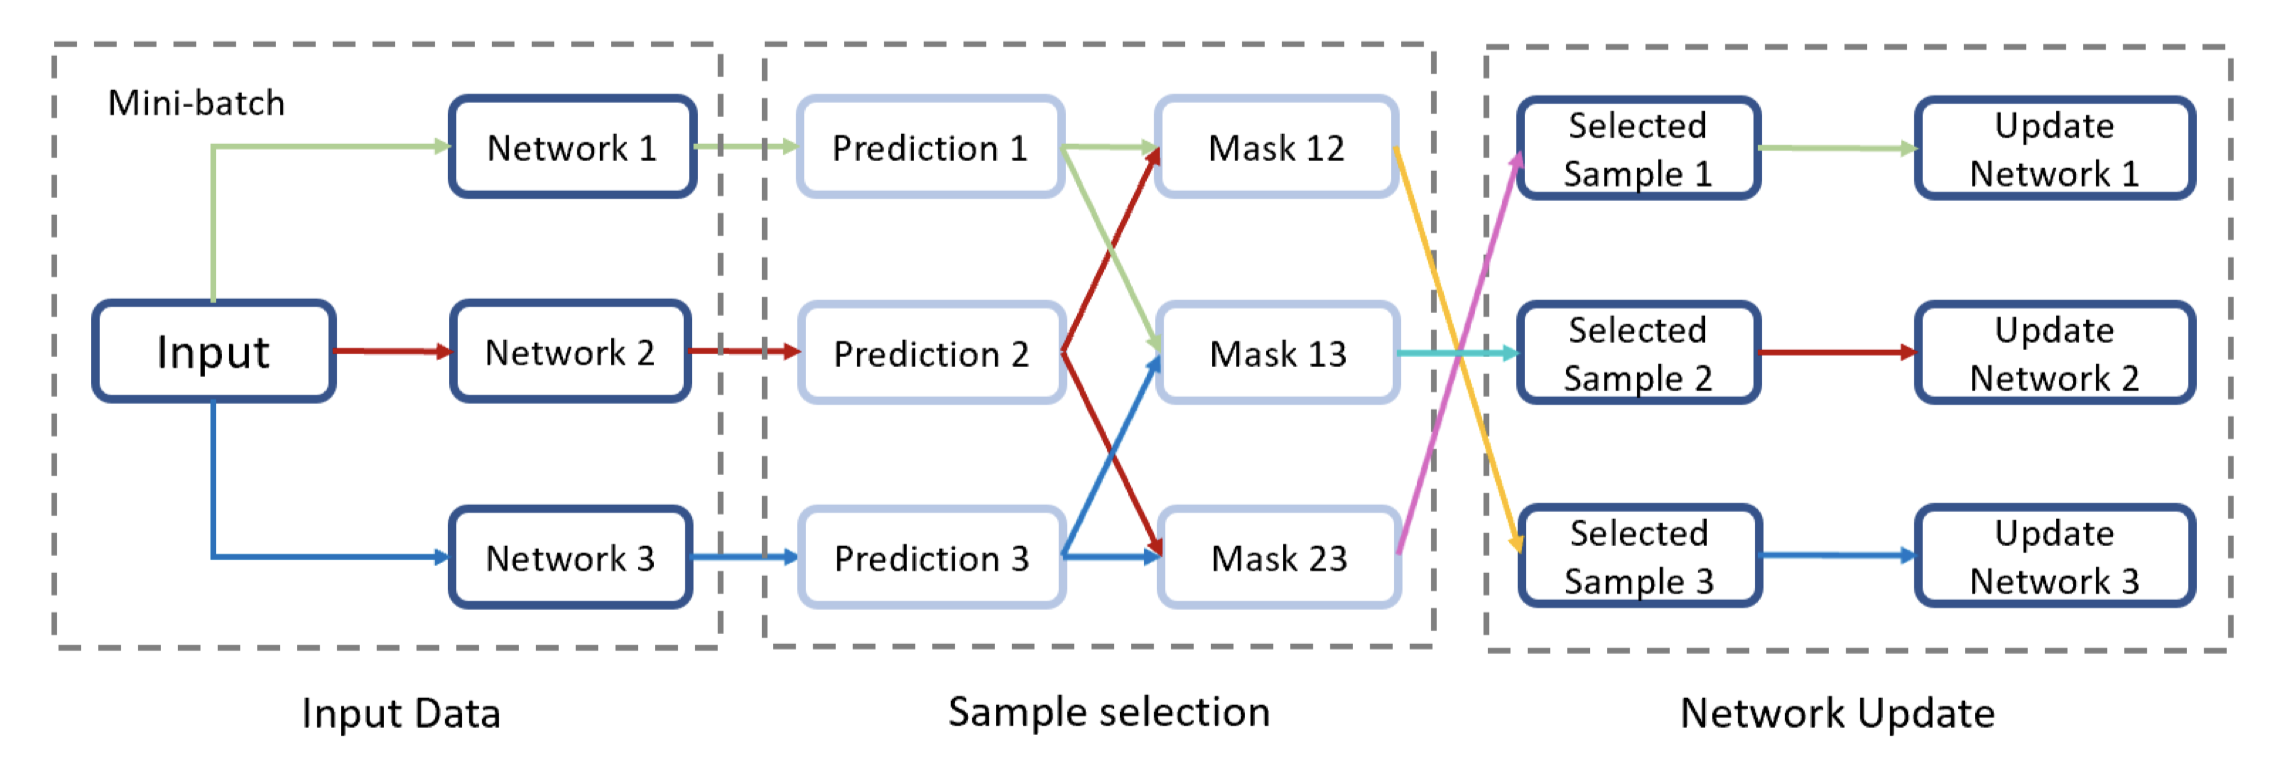
\includegraphics[width=1.0\textwidth]{img/c2/rel_c3.png}
        \bicaption{三网络协同教学框架,采用了像素级的样本选择策略。图自~\citet{Zhang2020RobustMI}。}{The pipeline of our Tri-network framework, which adopts the pixel-level sample selection strategy. Figure is from~\citet{Zhang2020RobustMI}.}
        \label{c2_fig13}
    \end{figure*}
模型框架如图~\ref{c2_fig13}所示,关键思想是同时训练三个网络,其中每一对网络都引导第三个网络从噪声标签中挖掘有用和可靠的信息。给定一个小批量的输入数据,分别送入三个网络,得到三种不同的预测图和相应的像素损失图。接下来,每一对网络根据其输出经样本选择策略选出可靠的像素,用以引导第三个网络的训练更新。在测试阶段,测试数据被送入三个训练好的网络,并将三个网络的输出合并后作为最终预测。

对于样本选择策略,该工作提出两种选择标准:基于共识的选择或基于差异的选择。这两个标准在处理有噪声标签的分割问题上都被证明是有效的。
基于共识的选择,是对网络预测的共识。对于每个小批数据,一对网络产生两组像素级预测图,通过计算网络预测和噪声标签之间每个像素的损失,可以得到每个网络相应的置信度图(也是损失图)。一个设置好的损失值阈值,会将每个置信度图二元化,其中 1 表示高置信度(对应小的损失值),0 表示低置信度(对应大的损失值)。基于两个网络的二元置信图,可以计算得到共识图。共识图中有两种像素:两个网络共同的高置信度像素(被认为有干净标签),和共同的低置信度像素(被认为难学习而有信息量的样本)。这两种像素被送入第三个网络训练,而其他不一致置信度的像素不予考虑。
基于差异的选择,与共识策略类似。首先计算每个网络预测的像素级损失图,然后计算两个损失图的差并取绝对值。在此策略中,通过选择一定比例的较大的损失差异像素,来挖掘有用的信息。选中的像素送入第三个网络更新其参数。


\section{本章小结}
本章中我们对相关的工作进行了总结与分析,包括基于弱标签的语义分割、自学习方法、去噪自编码器、基于噪声标签的语义分割等内容。为开展我们的研究奠定基础。

